%
% federgesetz.tex
%
% (c) 2021 Prof Dr Andreas Müller, OST Ostschweizer Fachhochschule
%
\documentclass[tikz]{standalone}
\usepackage{times}
\usepackage{amsmath}
\usepackage{txfonts}
\usepackage[utf8]{inputenc}
\usepackage{graphics}
\usetikzlibrary{arrows,intersections,math,calc}
\definecolor{darkred}{rgb}{0.8,0,0}
\usepackage{ifthen}
\begin{document}

\newboolean{showgrid}
\setboolean{showgrid}{false}
\def\breite{7}
\def\hoehe{4}

\def\l{0.75}
\def\R{10}
\pgfmathparse{(\l/\R)*(180/3.14159)}
\xdef\w{\pgfmathresult}

\begin{tikzpicture}[>=latex,thick]

\clip (-6.3,-3.4) rectangle (5.3,3.43);

% Povray Bild
\node at (-4.2,0) {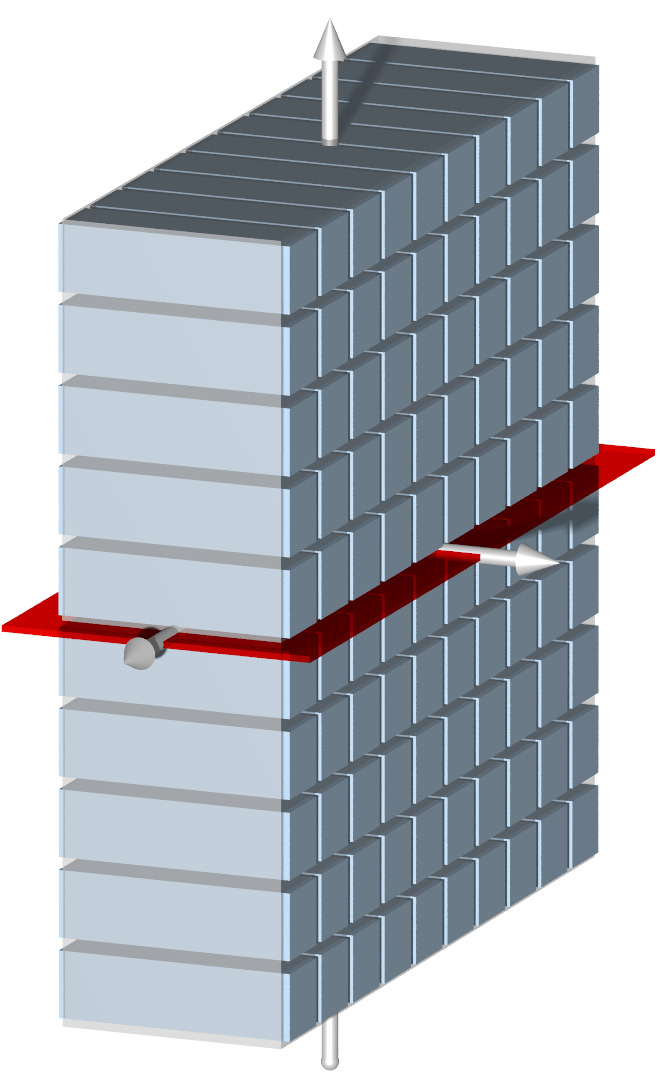
\includegraphics[width=4.2cm]{gerade.jpg}};
\node at (0,0) {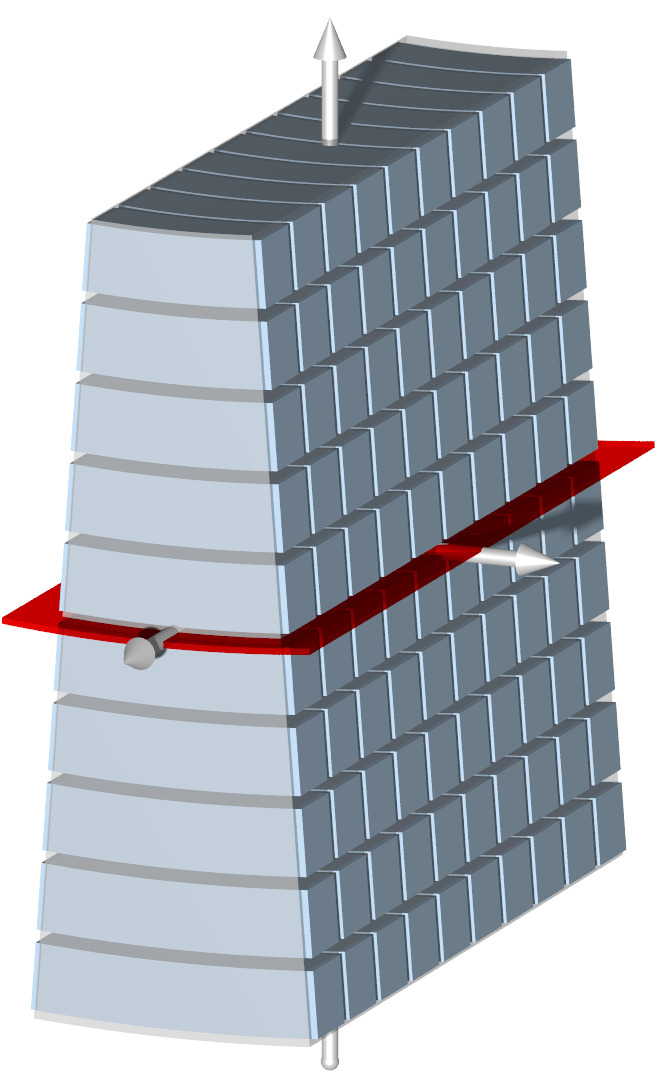
\includegraphics[width=4.2cm]{krumm.jpg}};

% Gitter
\ifthenelse{\boolean{showgrid}}{
\draw[step=0.1,line width=0.1pt] (-\breite,-\hoehe) grid (\breite, \hoehe);
\draw[step=0.5,line width=0.4pt] (-\breite,-\hoehe) grid (\breite, \hoehe);
\draw                            (-\breite,-\hoehe) grid (\breite, \hoehe);
\fill (0,0) circle[radius=0.05];
}{}

% Legende
\node at (-1.5,-0.8) {$z$};
\node at (-0.1,3.3) {$y$};
\fill[color=white,opacity=0.7] (1.5,-0.05) rectangle +(0.3,-0.3);
\node at ($(1.5,0)+(0.15,-0.2)$) {$x$};
\node at (-5.7,-0.8) {$z$};
\node at (-4.3,3.3) {$y$};
\fill[color=white,opacity=0.7] (-2.7,-0.05) rectangle +(0.3,-0.3);
\node at ($(-2.7,0)+(0.15,-0.2)$) {$x$};

%
%
\begin{scope}[xshift=4.2cm,yshift=-0.0cm]
	\clip (-1.1,-4) rectangle (1.1,4);
	\begin{scope}
		\clip (0,10) -- +({-90-\w}:12.5) arc({-90-\w}:{-90+\w}:12.5)
			-- cycle;
		\foreach \zi in {-5,-4,...,5}{
			\pgfmathparse{10-0.5*(\zi)}
			\xdef\r{\pgfmathresult}
			\fill[color=gray!60] (0,\R) circle[radius={\r+0.032}];
			\fill[color=blue!10] (0,\R) circle[radius={\r-0.032}];
		}
	\end{scope}
	\draw[color=darkred,line width=1.2pt] (0,\R) circle[radius=10];
	\fill[color=white] (0,\R) circle[radius=7.5];
	\draw[line width=0.3pt] ($(0,\R)+({-90-\w}:7.5)$) -- +(0,0.4);
	\draw[line width=0.3pt] ($(0,\R)+({-90+\w}:7.5)$) -- +(0,0.4);
	\draw[<->]
		($(0,\R)+({-90+\w}:7.5)+(0,0.3)$)
		--
		($(0,\R)+({-90-\w}:7.5)+(0,0.3)$);
	\node at (0,{5.6*0.5}) [above] {$\Delta x-w''(x)y$};
	\node[color=darkred] at (0,0) [above] {$\Delta x$};
	\draw[line width=0.3pt] ($(0,\R)+({-90-\w}:12.5)$) -- +(0,-0.4);
	\draw[line width=0.3pt] ($(0,\R)+({-90+\w}:12.5)$) -- +(0,-0.4);
	\draw[<->]
		($(0,\R)+({-90+\w}:12.5)+(0,-0.3)$)
		--
		($(0,\R)+({-90-\w}:12.5)+(0,-0.3)$);
	\node at (0,{-5.6*0.5}) [below] {$\Delta x-w''(x)y$};
\end{scope}

\end{tikzpicture}

\end{document}

